\documentclass{suribt}
\def\mbf#1{\mbox{\boldmath $#1$}} 
\def\rup#1{{^#1}\hspace{-0.5mm}}
%\documentclass[oneside]{suribt}% 本文が * ページ以下のときに (掲示に注意)
\usepackage{amsmath}
\usepackage[dvips]{graphicx}
\usepackage{cite}
%数式用の追加パッケージ
\usepackage{amsmath}
\usepackage{bm}

%\title{CLデータに基づく微小摺動制御法を用いたデスクトップ型NC工作機械}
\title{\huge Xtion Pro Liveカメラを用いた\\複数移動ロボットのビジュアルフィードバック制御の基礎実験計}
%\titlewidth{}% タイトル幅 (指定するときは単位つきで)
\author{三木 康平}
\eauthor{Hiroaki kurisu}% Copyright 表示で使われる
\studentid{F112026}
\supervisor{永田寅臣 教授}% 1 つ引数をとる (役職まで含めて書く)
%\supervisor{指導教員名 役職 \and 指導教員名 役職}% 複数教員の場合,\and でつなげる
\handin{2016}{03}% 提出月. 2 つ (年, 月) 引数をとる
%\keywords{キーワード1, キーワード2} % 概要の下に表示される
\begin{document}
\maketitle %%%%%%%%%%%%%%%%%%% タイトル %%%%
\frontmatter %ここから前文
\begin{abstract}%%%%%%%%%%%%% 概要 %%%%%%%%%%%%%%%%%%%%%


%%%%%%%%%%%%%%%%%%%%%%%%%%%%%%%%%%%%%%%%%%%%%%%%%%%%%%%%%


\end{abstract}
\tableofcontents%%%%%%%%%%%%% 目次 %%%%%%%%
\mainmatter% ここから本文 %%% 本文 %%%%%%%%
%%%%%%%%%%%%%%%%%%%%%%%%%%%%%%%%%%%%%%%%%%%%%%%%%%%%%%%%%%%%%%%%
%%%%%%%%%%%%%%%%%%%%%%%%%%%%%%%%%%%%%%%%%%%%%%%%%%%%%%%%%%%%%%%%
%%%%%%%%%%%%										%%%%%%%%%%%%
%%%%%%%%%%%%				第1章					%%%%%%%%%%%%
%%%%%%%%%%%%										%%%%%%%%%%%%
%%%%%%%%%%%%%%%%%%%%%%%%%%%%%%%%%%%%%%%%%%%%%%%%%%%%%%%%%%%%%%%%
%%%%%%%%%%%%%%%%%%%%%%%%%%%%%%%%%%%%%%%%%%%%%%%%%%%%%%%%%%%%%%%%
%%%%%%%%%%%%%%%%%%%%%%%%%%%%%%%%%%%%%%%%%%%
\chapter{緒言}
%%%%%%%%%%%%%%%%%%%%%%%%%%%%%%%%%%%%%%%%%%%
現在の商品生産方式はこれまでと大きく変わってきている. 高度経済成長期には, 大量生産で製造コストを下げ, 一般に普及させることが重要であった. このような少品種大量生産は, ラインの流れ作業による製造を生み, 同時に増加した繰り返し作業をロボットが代行することで自動化が図られた. 一方, 現在では消費者嗜好の多様化に合わせて変種変量生産が求められることが多くなってきた. 要求が常に変動するような作業は, ロボットを変化に応じて環境整備 ・ 作業教示 ・ 調整をする必要が生じるが, これでは採算が合わないため, 依然として工場制手工業が多く残る. したがって, 人のように状況判断を行い, 幅のある業務をこなすことができるような汎用機械としてのロボットが求められるようになってきている. 

汎用機械としてのロボットを目指すうえで, 重要なこととして井尻は次のように述べている.\\\\
"専用機械としてのロボットから汎用機械としてのロボットに生まれ変わるためには, 対象・環境・タスクに対する汎用性が重要である."\\\\
対象依存性をなくす研究としては, ロボット自身が試行錯誤に基づき動作を学習する深層学習や深層強化学習を用いたモデルが提案されている.


%%%%%%%%%%%%%%%%%%%%%%%%%%%%%%%%%%%%%%%%%%%%%%%%%%%%%%%%%%%%%%%%
%%%%%%%%%%%%%%%%%%%%%%%%%%%%%%%%%%%%%%%%%%%%%%%%%%%%%%%%%%%%%%%%
%%%%%%%%%%%%										%%%%%%%%%%%%
%%%%%%%%%%%%				第2章					%%%%%%%%%%%%
%%%%%%%%%%%%										%%%%%%%%%%%%
%%%%%%%%%%%%%%%%%%%%%%%%%%%%%%%%%%%%%%%%%%%%%%%%%%%%%%%%%%%%%%%%
%%%%%%%%%%%%%%%%%%%%%%%%%%%%%%%%%%%%%%%%%%%%%%%%%%%%%%%%%%%%%%%%
%%%%%%%%%%%%%%%%%%%%%%%%%%%%%%%%%%%%%%%%%%%%%%%%%%%%%%%%%%%%%%%%%%%%%%%%%%%%%
\chapter{運動学}
%%%%%%%%%%%%%%%%%%%%%%%%%%%%%%%%%%%%%%%%%%%%%%%%%%%%%%%%%%%%%%%%%%%%%%%%%%%%%
ロボットアームの手先を目的の位置に移動させたいとき, 各関節角度と関節間の長さ現在の手先位置が分かっていれば, 運動学を用いて必要な姿勢を計算することが出来る. 運動学とは, ロボットアームの関節角度や関節間の長さと手先位置・姿勢の関係を数式で表したものであり, 各関節角度から手先位置・姿勢を求めることを順運動学, 手先位置・姿勢から各関節角度を求めることを逆運動学という. 
また, ロボットアームは各関節ごとに座標系(関節座標系)を設定することができ, この座標系と台座部に設定した基準座標系は運動学に用いることで互いに変換することができる.

%%%%%%%%%%%%%%%%%%%%%%%%%%%%%%%%%%%%
\section{順運動学}
%%%%%%%%%%%%%%%%%%%%%%%%%%%%%%%%%%%%
順運動学とは, ロボットアームの各関節角度から手先位置・姿勢を求めること, すなわち手先位置の関節座標系から基準座標系への変換ということができる. ここでは関節座標の手先位置を基準座標系に変換する方法について示す. まず簡単のために図\ref{fig:translation}のような系の並進移動について考える.
%------------
%Figure translation
%------------
\begin{figure}[ht]
 \begin{center}
  \includegraphics[width=60mm,clip]{./figure/translation.eps}
  \caption{Polishing scene using a conventional industrial robot with a servo spindle.}
  \label{fig:translation}
 \end{center}
\end{figure}

移動後の原点$O'(x_0', y_0', z_0')$は, 移動前の原点$O(x_0, y_0, z_0)$から見ると次のように表される.
%------------
%数式 並進移動_1
%------------
\begin{eqnarray*}
	x_0' = x_0 + x_1 \\
	y_0' = y_0 + y_1 \\
	z_0' = z_0 + z_1
\end{eqnarray*}

上式をベクトル${\bm r}$を用いて表すと, 以下のようになる.
%------------
%数式 並進移動_ベクトル
%------------
\begin{equation}
	\label{O-O'translation}
	O' = O + {\bm r}
\end{equation}

関節座標系から基準座標系への変換を行うには、並進移動だけでなく回転移動についても考える必要がある. そこで図\ref{fig:1rink}のような簡単な系の回転移動について考える.
%------------
%Figure 1rink
%------------
\begin{figure}[ht]
 \begin{center}
  \includegraphics[width=60mm,clip]{./figure/1rink.eps}
  \caption{Polishing scene using a conventional industrial robot with a servo spindle.}
  \label{fig:1rink}
 \end{center}
\end{figure}

 まずベクトル${\bm P}(x_1, y_1, z_1)$は, 各軸方向の単位ベクトル(${\bm i}, {\bm j}, {\bm k}$)を用いて次のように表される.
%------------
%Pベクトル
%------------
\begin{equation}
	\label{Pvector}
	{\bm P} = x_1{\bm i} + y_1{\bm j} + z_1{\bm k}
\end{equation}

次に, Z軸を基準としてベクトル${\bm P}$を含むX-Y平面を$\theta$だけ回転した座標系を新しく$X', Y', Z'$座標系とすると, その座標系におけるとすると, ベクトル${\bm P'}(x_2, y_2, z_2)$は単位ベクトル${\bm i'}, {\bm j'}, {\bm k'}$を用いて次のように表される.
%------------
%P'ベクトル
%------------
\begin{equation}
	\label{P'vector}
	{\bm P'} = x_2{\bm i'} + y_2{\bm j'} + z_2{\bm k'}
\end{equation}

ここで, 単位ベクトル単位ベクトル${\bm i'}, {\bm j'}, {\bm k'}$は回転前の座標系から見ると

%------------
%単位ベクトルの回転行列
%------------
\begin{equation}
	\label{RotationMatrix}
	\left[
		\begin{array}{c}
			{\bm i'} \\
			{\bm j'} \\
			{\bm k'}
		\end{array}
	\right]
	=
	\left[
		\begin{array}{ccc}
			\cos \theta & \sin \theta & 0 \\
			-\sin \theta & \cos \theta & 0 \\
			0                & 0                 & 0
		\end{array}
	\right]
	\left[
		\begin{array}{c}
			{\bm i} \\
			{\bm j} \\
			{\bm k}
		\end{array}
	\right]
\end{equation}

と表せる. さらに式(\ref{RotationMatrix})に式(\ref{P'vector})と式(\ref{Pvector})を代入すると

%------------
%単位ベクトルの回転行列
%------------
\begin{eqnarray*}
	\left[
		\begin{array}{c}
			x_2 \\
			y_2 \\
			z_2
		\end{array}
	\right]
	=
	\left[
		\begin{array}{ccc}
			\cos \theta & \sin \theta & 0 \\
			-\sin \theta & \cos \theta & 0 \\
			0                & 0                 & 0
		\end{array}
	\right]
	\left[
		\begin{array}{c}
			x_1 \\
			y_1 \\
			z_1
		\end{array}
	\right]
\end{eqnarray*}

さらに見通しをよくするため, 単位ベクトルを省略し以下のように表す.


%------------
%単位ベクトルの回転行列
%------------
\begin{equation}
	\label{P-P'RotationMatrix}
	{\bm P'}
	=
	\left[
		\begin{array}{ccc}
			\cos \theta & \sin \theta & 0 \\
			-\sin \theta & \cos \theta & 0 \\
			0                & 0                 & 0
		\end{array}
	\right]
	{\bm P}
\end{equation}

 すなわちZ軸を基準としたベクトルの回転移動は, 移動前後の位置移動および相対角$\theta$を用いて表すことができ, これはX軸, Y軸においても成り立つ. この式(\ref{P-P'RotationMatrix})中央の行列を回転行列といい$R$で表すこととする. 
並進移動と回転移動とを用いることにより, 図\ref{fig:ComplexTransform}に示すような一見複雑な座標系の変換も次のような式で表すことができる.

%------------
%Figure ComplexTransform
%------------
\begin{figure}[ht]
 \begin{center}
  \includegraphics[width=60mm,clip]{./figure/ComplexTransformation.eps}
  \caption{Polishing scene using a conventional industrial robot with a servo spindle.}
  \label{fig:ComplexTransform}
 \end{center}
\end{figure}

%------------
%座標変換の一般式
%------------
\begin{equation}
	^{A}{\bm P} = {^{A}{\bm R}_B}{^{B}{\bm P}} + ^{A}{\bm r}_B
\end{equation}

 ここで${^{A}{\bm R}_B}$は座標系Aから座標系Bへの回転行列である. この関係を各関節ごとに用いることで, 手先位置を基準座標系からの位置として求めることができる.

%%%%%%%%%%%%%%%%%%%%%%%%%%%%%%%%%%%%
\section{逆運動学}
%%%%%%%%%%%%%%%%%%%%%%%%%%%%%%%%%%%%
順運動学が座標変換を行うことで解が1つ求まるのに対して, 逆運動学では図\ref{fig:InverseKinematics}の場合のように手先位置が同じ位置にある場合でも各リンクの位置と姿勢にはいくつかの解が存在することや, 解自体が存在しないこともある. このような問題があるため, 一般に順運動学より逆運動学の方が問題を解くのが難しい.
%------------
%Figure Inverse kinematics
%------------
\begin{figure}[ht]
 \begin{center}
  \includegraphics[width=40mm,clip]{./figure/InverseKinematics.eps}
  \caption{Polishing scene using a conventional industrial robot with a servo spindle.}
  \label{fig:InverseKinematics}
 \end{center}
\end{figure}

%------------
%Figure 2rink
%------------
\begin{figure}[ht]
 \begin{center}
  \includegraphics[width=60mm,clip]{./figure/2rink.eps}
  \caption{Polishing scene using a conventional industrial robot with a servo spindle.}
  \label{fig:2rink}
 \end{center}
\end{figure}

逆運動学でアームの関節角度を計算する例として, 図\ref{fig:2rink}のような場合を考える. まず, 角度$\alpha$と$|{\bm {OP}}|$の関係は余弦定理を用いて次式で表される.
%------------
%数式 2リンクの手先位置_1
%------------
\begin{equation}
		\label{alpha-OPRelationship}
		\cos \alpha = \frac{L^2_1 + L^2_2 - |{\bm {OP}}|}{2 L_1 L_2}
\end{equation}

式(\ref{alpha-OPRelationship})より角度$\alpha$は$\alpha = \cos^{-1}(\cos \alpha)$と表せるので, 結果的に$\theta_2$は次式で表される.
%------------
%数式 θ2と角度αとの関係
%------------
\begin{equation}
	\theta_2 = \pi - \alpha
\end{equation}

同様に, 余弦定理を用いて角度$\beta$と$|OP|$の関係は次式で表され,
%------------
%数式 角度βと補助線OPとの関係
%------------
\[
	\cos \beta = \frac{|{\bm {OP}}|^2 + L^2_1 - L^2_2}{2 |{\bm {OP}}| L_2}
\]

$\beta = \cos^{-1}(\cos \beta)$である. 最後に角度$\gamma$は, 補助線$|{\bm OP}|$と手先位置のx座標との関係から
%------------
%数式 角度γと補助線OPとの関係
%------------
\[
	\cos \gamma = \frac{x}{|{\bm {OP}}|}
\]

であるので, $\gamma = \cos^{-1}(\cos \gamma)$ である. よって, 角度$\beta$および角度$\alpha$を用いて$\theta_1$は次式で表される.
\begin{equation}
	\theta_1 = \gamma - \beta
\end{equation}

よって, 手先位置から関節角度$\theta_1$, $theta_2$を求めることができた.

%------------
%Figure 2rink_2
%------------
\begin{figure}[ht]
 \begin{center}
  \includegraphics[width=60mm,clip]{./figure/2rink_2.eps}
  \caption{Polishing scene using a conventional industrial robot with a servo spindle.}
  \label{fig:2rink_2}
 \end{center}
\end{figure}

また別の方法として, 図\ref{fig:2rink_2}のような場合を考える. この場合, 手先位置は次式で表される.
%------------
%数式 2リンクの手先位置_2
%------------
\begin{align}
	\begin{aligned}
		\label{ForwardKinematicEquation}
		x_p = l_1 \cos \theta_1 + l_2 \cos(\theta_1 + \theta_2) \\
		y_p = l_1 \sin \theta_1 + l_2 \sin(\theta_1 + \theta_2) 
	\end{aligned}
\end{align}

式(\ref{ForwardKinematicEquation})の両辺を時間で微分し, 行列で表すと
%------------
%数式 手先位置の速度と各関節の角速度の関係
%------------
\begin{equation}
	\label{ForwardKinematicEquation_diff}
	\frac{d{\bm P}}{dt} = {\bm J}({\bm \theta})\frac{d{\bm \theta}}{dt}
\end{equation}

ここで
%------------
%数式 手先位置の速度と各関節の角速度の関係の変数
%------------
\[
{\bm P} = \left[x_p, y_p \right]^{\mathrm{T}}, {\bm \theta} = \left[\theta_1, \theta_2\right]^{\mathrm{T}}, 
{\bm J}({\theta}) = 
	\left[
		\begin{array}{cc}
			-(l_1 \sin \theta_1 + l_2 \sin(\theta_1 + \theta_2) & -l_2 \sin(\theta_1 + \theta_2) \\
			l_1 \cos \theta_1 + l_2 \cos(\theta_1 + \theta_2) & l_2 \cos(\theta_1 + \theta_2)
		\end{array}
	\right]
\]

である. 式(\ref{ForwardKinematicEquation_diff})は手先位置の速度と各関節における角速度の関係を表しており, 両辺の変換を担う行列${\bm J}$を一般にヤコビ行列という. 
さて, 逆運動学は手先位置から各関節角度を求める問題のことであったので, 式(\ref{ForwardKinematicEquation_diff})を以下のように変形する.
%------------
%数式 ヤコビ行列の逆行列
%------------
\begin{equation}
	\label{ForwardKinematicEquation_diff}
	\frac{d{\bm \theta}}{dt} = {\bm J}^{-1}\frac{d{\bm P}}{dt}
\end{equation}

しかし, ${\bm J^{-1}}$は必ずしも存在しない. ${\bm J^{-1}}$が存在しない条件は, det${\bm J^{-1}}$で求めることができ, その時の姿勢を特異姿勢もしくは特異点という. 


%%%%%%%%%%%%%%%%%%%%%%%%%%%%%%%%%%%%%%%%%%%%%%%%%%%%%%%%%%%%%%%%
%%%%%%%%%%%%%%%%%%%%%%%%%%%%%%%%%%%%%%%%%%%%%%%%%%%%%%%%%%%%%%%%
%%%%%%%%%%%%										%%%%%%%%%%%%
%%%%%%%%%%%%				第3章					%%%%%%%%%%%%
%%%%%%%%%%%%										%%%%%%%%%%%%
%%%%%%%%%%%%%%%%%%%%%%%%%%%%%%%%%%%%%%%%%%%%%%%%%%%%%%%%%%%%%%%%
%%%%%%%%%%%%%%%%%%%%%%%%%%%%%%%%%%%%%%%%%%%%%%%%%%%%%%%%%%%%%%%%
%%%%%%%%%%%%%%%%%%%%%%%%%%%%%%%%%%%%%%%%%%%%%%%%%%%%%%%%%%%%%%%%%%%%%%%%%%%%%
\chapter{ニューラルネットワーク}
%%%%%%%%%%%%%%%%%%%%%%%%%%%%%%%%%%%%%%%%%%%%%%%%%%%%%%%%%%%%%%%%%%%%%%%%%%%%%

%%%%%%%%%%%%%%%%%%%%%%%%%%%%%%%%%%%%
\section{人工知能}
%%%%%%%%%%%%%%%%%%%%%%%%%%%%%%%%%%%%





%%%%%%%%%%%%%%%%%%%%%%%%%%%%%%%%%%%%
\section{機械学習}
%%%%%%%%%%%%%%%%%%%%%%%%%%%%%%%%%%%%



%%%%%%%%%%%%%%%%%%%%%%%%%%%%%%%%%%%%
\section{ニューラルネットワーク}
%%%%%%%%%%%%%%%%%%%%%%%%%%%%%%%%%%%%



%%%%%%%%%%%%%%%%%%%%%%%%%%%%%%%%%%%%%%%%%%%%%%%%%%%%%%%%%%%%%%%%
%%%%%%%%%%%%%%%%%%%%%%%%%%%%%%%%%%%%%%%%%%%%%%%%%%%%%%%%%%%%%%%%
%%%%%%%%%%%%										%%%%%%%%%%%%
%%%%%%%%%%%%				第4章					%%%%%%%%%%%%
%%%%%%%%%%%%										%%%%%%%%%%%%
%%%%%%%%%%%%%%%%%%%%%%%%%%%%%%%%%%%%%%%%%%%%%%%%%%%%%%%%%%%%%%%%
%%%%%%%%%%%%%%%%%%%%%%%%%%%%%%%%%%%%%%%%%%%%%%%%%%%%%%%%%%%%%%%%
%%%%%%%%%%%%%%%%%%%%%%%%%%%%%%%%%%%%%%%%%%%%%%%%%%%%%%%%%%%%%%%%%%%%%%%%%%%%%
\chapter{実機による動作実験}
%%%%%%%%%%%%%%%%%%%%%%%%%%%%%%%%%%%%%%%%%%%%%%%%%%%%%%%%%%%%%%%%%%%%%%%%%%%%%

%%%%%%%%%%%%%%%%%%%%%%%%%%%%%%%%%%%%
\section{Dobot}
%%%%%%%%%%%%%%%%%%%%%%%%%%%%%%%%%%%%
TechShare社が販売しているDobot Magician(Dobot)は, 4自由度のロボットアームでありエンドエフェクタを取り換えることによって3Dプリンタのような積載加工, エンドミルによる切削加工ペンツールを使った印字などが行える. 
Dobotの質量と可搬質量はそれぞれ3.4kgと500gであり, 位置繰り返し精度は0.2mmと教育ロボットとしては優れている. 
またDobot社より, CやMFC(Microsoft Foundation Class), Pythonなど複数のプログラミング言語でAPIが提供されており, 個人でプログラムを組む際の敷居も低い. 
今回は, その中のPython APIを統合開発環境であるVisual Studio2019上に実装し, Dobot本体を動作させるプログラムの開発を行った. APIとはあるコンピュータプログラム(ソフトウェア)の機能や管理するデータなどを、外部の他のプログラムから呼び出して利用するための手順やデータ形式などを定めた規約のことである. 
今回はその中からDobot本体の姿勢を取得するためのGetPose()
また, Pythonに標準で搭載されているGUI作成キットであるTkinterを用いて, 開発した動作プログラムを簡単に扱えるようDobot制御用のユーザインタフェースの作成も行った. 

%%%%%%%%%%%%%%%%%%%%%%%%%%%%%%%%%%%%
\section{学習データ}
%%%%%%%%%%%%%%%%%%%%%%%%%%%%%%%%%%%%

%%%%%%%%%%%%%%%%%%%%%%%%%%%%%%%%%%%%
\section{実験結果}
%%%%%%%%%%%%%%%%%%%%%%%%%%%%%%%%%%%%


%%%%%%%%%%%%%%%%%%%%%%%%%%%%%%%%%%%%%%%%%%%%%%%%%%%%%%%%%%%%%%%%
%%%%%%%%%%%%%%%%%%%%%%%%%%%%%%%%%%%%%%%%%%%%%%%%%%%%%%%%%%%%%%%%
%%%%%%%%%%%%										%%%%%%%%%%%%
%%%%%%%%%%%%				第5章					%%%%%%%%%%%%
%%%%%%%%%%%%										%%%%%%%%%%%%
%%%%%%%%%%%%%%%%%%%%%%%%%%%%%%%%%%%%%%%%%%%%%%%%%%%%%%%%%%%%%%%%
%%%%%%%%%%%%%%%%%%%%%%%%%%%%%%%%%%%%%%%%%%%%%%%%%%%%%%%%%%%%%%%%
%%%%%%%%%%%%%%%%%%%%%%%%%%%%%%%%%%%%%%%%%%%%%%%%%%%%%%%%%%%%%%%%%%%%%%%%%%%%%
\chapter{今後の方針}
%%%%%%%%%%%%%%%%%%%%%%%%%%%%%%%%%%%%%%%%%%%%%%%%%%%%%%%%%%%%%%%%%%%%%%%%%%%%%









\backmatter% ここから後付
\chapter{謝辞}%%%%%%%%%%%%%%% 謝辞 %%%%%%%
本研究は,山口東京理科大学大学院基礎工学研究科基礎工学専攻で行われたものである.
\begin{thebibliography}{}%%%参考文献%%%%%%
\bibitem{Suzuki-2018}
鈴木真太郎, 永田寅臣, 渡辺 桂吾 ``多関節ロボットのためのCAD/CAMインタフェイス", 日本機械工学会九州支部北九州講演会講演論文集, No. 188-3, 2018.

\bibitem{Borangiu-2010}
T. Borangiu, F.D. Anton and S. Anton, ``Open architecture for robot controllers,'' {\it Procs. of 2010 IEEE 19th International Workshop on Robotics in Alpe-Adria-Danube Region (RAAD)}, pp. 181--186, 2010.

\bibitem{Ying-2011}
Z. Ying, W. Tianmiao, W. Hongxing, L. Miao, ``Robot software architecture based on IPv6,'' {\it Procs. of 6th IEEE Conference on Industrial Electronics and Applications}, pp. 1666--1671, 2011.

\bibitem{Mizukawa-2001}
水川 真,尾崎安男,``産業用ロボットにおけるネットワークインタフェースの標準化活動", 東芝レビュー,Vol. 56, No. 9, pp. 7--11, 2001.

\bibitem{Mizukawa-2001-2}
M. Mizukawa, T. Koyama, T. Inukai, A. Noda, N. Kanamaru, Y. Noguchi, and N. Otera, ``Proposal of open-network-interface for industrial robots (ORiN) and its experimental evaluation,'' {\it Procs. of 2001 IEEE/ASME International Conference on Advanced Intelligent Mechatronics}, pp.  689--694, 2001.

\bibitem{Mizukawa-2002}
M. Mizukawa, H. Matsuka, T. Koyama, T. Inukai, A. Noda, H. Tezuka, Y. Noguchi, and N. Otera, ``ORiN: open robot interface for the network-- the standard and unified network interface for industrial robot applications,'' {\it Procs. of the 41st SICE Annual Conference}, pp.  925--928, 2002.

\bibitem{Mizukawa-2004}
M. Mizukawa, S. Sakakibara, and N. Otera, ``Implementation and applications of open data network interface ORiN,'' {\it Procs. of the 43rd SICE Annual Conference}, pp. 1340--1343, 2004.

\bibitem{Nagata-2000}
永田寅臣,渡辺桂吾,泉 清高,``多軸制御用CLデータに基づく位置補償器を用いた産業用ロボットの倣い制御",精密工学会誌, Vol. 66, No. 3, pp. 473--477, 2000.

\bibitem{Nagata-2013-1}
F. Nagata and K. Watanabe,
{\it Controller Design for Industrial Robots and Machine Tools: Applications to Manufacturing Processes},
Woodhead Publishing, UK, 2013.

%\bibitem{Interior-2006}
%http://www.fitc.pref.fukuoka.jp/

\bibitem{Nagata-2007}
F. Nagata, Y. Kusumoto, Y. Fujimoto, and K. Watanabe, ``Robotic sanding system for new designed furniture with free-formed surface,''
{\it Robotics and Computer-Integrated Manufacturing},
Vol. 23, No. 4, pp. 371--379, 2007.

\bibitem{Nagata-2014}
F. Nagata, A. Otsuka, K. Watanabe and Maki K. Habib, ``Fuzzy feed rate controller for a machining robot,'' {\it Procs. of the 2014 IEEE International Conference on Mechatronics and Automation (IEEE ICMA 2014)}, pp. 198--203, 2014.


\bibitem{VE026A}
VE026A ORiN Option Users' Guide, Version 1.0.0, DENSO WAVE Inc., December 14th, 2012.

\bibitem{ORiN2}
ORiN2 Programming Guide, Version 1.0.12.0, DENSO WAVE Inc., September 7th, 2012.




\end{thebibliography}


\end{document}


